\documentclass[a4paper]{article}
\usepackage[pdftex]{graphicx}
\usepackage[utf8]{inputenc}
\usepackage{enumerate}
\usepackage{siunitx}
\sisetup{locale=DE}
\usepackage{icomma}
\usepackage{amssymb}
\usepackage{tikz}
\usepackage{href-ul}
\hypersetup{
	colorlinks=true,
	linkcolor=blue,
	urlcolor=blue}
\usepackage{geometry}
\geometry{a4paper, top=15mm, left=15mm, right=15mm, bottom=15mm,
	headsep=10mm, footskip=12mm}

\begin{document}
	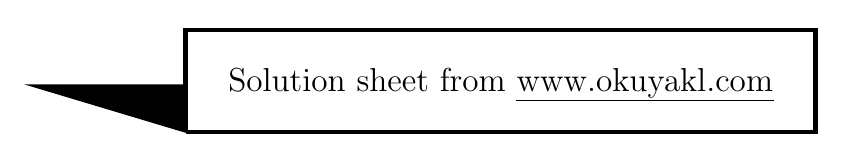
\begin{tikzpicture}(10,3)
		\draw[ultra thick](2,0) --(10,0) -- (10,1.3) --(2,1.3) -- (2,0);
		\draw[fill=black](2,0)-- (0,.6) -- (2,.6) -- (2,0);
		\node at (6,.6) {\large Solution sheet from \href{http://www.okuyakl.com}{www.okuyakl.com}};
	\end{tikzpicture}
	\vspace{0.5 cm}
	
	
	\noindent {\bf Task 1.}\\
	During charging, a voltage builds up in the capacitor that counteracts the applied voltage. That's why the charging current is initially large and then decreases exponentially.
	\vspace{0.5 cm}
	
	\noindent {\bf Task 2.}\\
	The bead is attracted to the positively charged plate of the capacitor. On its way there it covers the distance $d/2$. The acting Coulomb force $F_C$ does the work
	$$W_{el} = F_C \cdot {d \over 2}$$ which we equate with the kinetic energy $E_{kin}$ of the bead and solve for $v(d)$:
	
	$$
	\renewcommand{\arraystretch}{2}
	\begin{array}{rcll}
		W_{el} & = & E_{kin} \\
		F_C \cdot {d \over 2} & = & {1 \over 2}m v(d)^2 \\
		q \cdot E \cdot {d \over 2} & = & {1 \over 2}m v(d)^2 & | \cdot 2 : m \\
		{q \cdot E \cdot d \over m} & = & v(d)^2 & | \sqrt{\quad}\\
		v(d) & = & \sqrt{q \cdot E \cdot d \over m} &|(*) \\
		v(d) & = & \sqrt{q \cdot E \over m} \cdot \sqrt{d} \\
		v(d) & = & \sqrt{\SI{1,4e-9}{\coulomb} \cdot \SI{36e3}{\volt\over \meter}\over \SI{12e-6}{\kilogram }} \cdot \sqrt{d}\\
		& = & 2.0 \cdot \sqrt{\SI{}{\coulomb \cdot \volt \over \kilogram \cdot \meter}} \cdot \sqrt{d} \\
		& = & 2.0 \cdot \sqrt{ \SI{}{\joule \over \kilogram \cdot \meter}} \cdot \sqrt{d}\\
		& = & 2.0 \cdot \sqrt{\SI{}{{\kilogram \cdot \meter^2 \cdot \second^{-2}} \over {\kilogram \cdot \meter}}} \cdot \ sqrt{d}\\
		& = & \SI{2,0}{\sqrt{\meter}\over \second} \cdot \sqrt{d}
	\end{array}
	$$
	\vspace{0.5 cm}
	
	\noindent {\bf Task 3.}\\
	The following applies to the voltage:
	$$ U = E \cdot d $$
	We replace the factor $E \cdot d $ from $(*)$ with $U$:
	$$ v = \sqrt{q \cdot U \over m} \quad (**)$$
	We then solve for the tension and insert:
	$$
	\renewcommand{\arraystretch}{2}
	\begin{array}{rcl}
		U & = & {v^2 \cdot m \over q} \\
		& = & {(\SI{0.56}{\meter\over \second})^2 \cdot \SI{12e-6}{\kilogram} \over \SI{1.4e-9}{\coulomb }}\\
		& = & \SI{2688}{\volt}\\
		& = & \SI{2.7}{\kilo\volt}
	\end{array}
	$$
	Unit check:
	
	$$\SI{}{\meter^2\cdot \second^{-2}\kilogram \over \coulomb}=\SI{}{\joule\over \coulomb}=\SI{}{\volt}$$
	\vspace{0.5 cm}
	
	\noindent {\bf Task 4.}\\
	The plate spacing $d$ no longer appears in the formula $(**)$;
	With an existing connection to the voltage source, $U$ remains constant, so $v$ does not change.
	\vspace{0.5 cm}
	
	\noindent {\bf Task 5.}\\
	When it comes into contact with the positively charged plate, the bead also becomes positively charged and is consequently repelled. Now the Coulomb force acts in the other direction and the bead moves to the negative plate, where it is charged again, changes direction and so on...
	
	\begin{center}
		\includegraphics[width=7 cm]{../../viecher/eendcomic.pdf}
		
		Here you can go back to the \href{https://www.okuyakl.de/phys/p12efeldL093/ae093.pdf}{Task sheet}
	\end{center}
	
\end{document}